\chapter{Testing and Benchmarking}
In this chapter, we describe how our platform is verified and validated. Then, we measured the performance of the database system with different count of clients, and we compared results with other database systems. 


\section{Testing}
Testing is an essential part of the development of any project. As part of my master thesis, We~performed two types of testing. Unit testing to ensure that every platform module works correctly, and testing the user interface of ExplorerGUI in which we~tested how quickly and efficiently the user handles tasks, and how user-friendly the user interface is.

\begin{figure}[h]
    \centering
    \begin{lstlisting}[style=ES6]
describe("Btree", () =>
{
    it("insert values to btree", async () =>
    {
        const t = new BTree();
        for (let i = 0; i < 100; i++)
        {
            await t.add(i, { name: "test object", value: i });
        }

        for (let i = 0; i < 100; i++)
        {
            expect(await t.find(i)).toStrictEqual({ name: "test object", value: i });
        }
        expect(await t.find(101)).toBe(null);
    });
});
    \end{lstlisting}
    \caption{Unit test for B-Tree insert operation.}
    \label{unitTest}
\end{figure}

\subsection{Unit Testing}
We tested all critical parts of the Explorer-core module through unit tests. We use jest.js\footnote{\url{https://jestjs.io/}} framework for writing tests. We test every operation on B-Tree index (add, remove, find, update), an append-only log that is used for database log and record log (add, merge, difference). Test for B-Tree insert operation can be seen in Figure \ref{unitTest}. Tests for every application we have developed in this thesis can be run by command \texttt{npm run test}.






% \subsection{Testing of User Interface}
% We also test ExplorerGUI by a user. We invited for this type of testing five people whose task was to perform several simple steps:
% \begin{enumerate}
%     \item Load ExplorerGUI web page.
%     \item Select cryptocurrency.
%     \item Make filter that selects all blocks between 1,000 and 2,000.
%     \item Click on any block to view its transactions.
%     \item Select some address and view its transactions.
% \end{enumerate}
% There were almost no problems during testing. As this is a relatively complex platform that requires at least a minimum knowledge of cryptocurrencies, the principles of blocks and transactions were not clear to all tested. However, testers completed the tasks in a short time. The user interface seemed to everyone intuitive and straightforward. Subsequently, given the test results, we performed a few graphical changes, such as enlarging and highlighting some controls. Also, most testers liked the graphic design and the chosen colours of the application.




\section{Benchmarking}
\label{benchmark}
To test the performance of our platform, we have focused on the speed of transaction processing in the database system. We compared our database system to other widely used solutions -- MySQL and PostgreSQL.



\subsubsection{MySQL}
MySQL is leading open-source multi-platform relational database system. Originally, MySql was created by the Swedish company MySQL AB, now owned by Oracle Corporation. It can provide stable and robust database solution for application. Due to its easy deployment, performance and especially due to the fact that it is a freely distributable software, it has a high share in currently used databases. 
\cite{mysql2001mysql, dubois1999mysql}

\subsubsection{PostgreSQL}
PostgreSQL is object-relational widly used open-source database system. It is available for Linux, FreeBSD, OpenBSD, and Windows. PostgreSQL was formed in 1977. Project started in university of California and later on was developed commercially. To this date PostgreSQL has active development wordwide community. Main advantage of PostgreSQL is aprouch of object-relational model. This allows developers to store. It is designed to handle a range of workloads, from single machines to data warehouses or Web services with many concurrent users. \cite{drake2002practical}

\subsubsection{Environment}
We compare MySQL and PostgresSQL with our peer-to-peer database system. These database systems run virtualized in Docker containers on hardware with 4 cores processor Intel Pentium G4560 3.50GHz and 16 GB of RAM.  We start clients that connect to these database systems and performs queries on different hardware. Then we measure average queries per seconds that clients execute. Clients are written in JavaScript with official node.js connectors for MySQL\footnote{\url{https://www.npmjs.com/package/mysql}} and PostgreSQL\footnote{\url{https://www.npmjs.com/package/postgres}} and are connected in the LAN with database systems over 1Gb Ethernet. Database structure that is used in benchmarks can be seen in Figure \ref{benchDatabaseStructure}. Table \texttt{authors} contains 10,000 records and table \texttt{posts} contains 50,000 records (each author has 5 posts). Test query for each database system can be seen in Figure \ref{benchQuery}.

\begin{figure}[h]
    \begin{subfigure}[t]{.3\textwidth}
        \begin{lstlisting}[language=SQL,basicstyle=\tiny]
            CREATE TABLE `authors` (
                `id` int(11) PRIMARY KEY,
                `first_name` varchar(50),
                `last_name` varchar(50),
                `email` varchar(100),
                `birthdate` date,
                `added` timestamp,
                PRIMARY KEY (`id`),
                UNIQUE KEY `email` (`email`)
            );

            CREATE TABLE `posts` (
                `id` int(11) PRIMARY KEY,
                `author_id` int(11),
                `title` varchar(255),
                `description` varchar(500),
                `content` text,
                `date` date,
                PRIMARY KEY (`id`)
            );
        \end{lstlisting}
        \caption{MySQL}
    \end{subfigure}%
    \begin{subfigure}[t]{.3\textwidth}
        \begin{lstlisting}[language=SQL,basicstyle=\tiny]
            CREATE TABLE authors (
                id serial PRIMARY KEY,
                first_name varchar(50),
                last_name varchar(50),
                email varchar(100),
                birthdate date,
                added timestamp
            );

            CREATE TABLE posts (
                id serial PRIMARY KEY,
                author_id integer,
                title varchar(255),
                description varchar(500),
                content text,
                date date
            );
        \end{lstlisting}
        \caption{PostgreSQL}
    \end{subfigure}
    \begin{subfigure}[t]{.3\textwidth}
        \begin{lstlisting}[style=ES6,basicstyle=\tiny]
            class Author {
                @PrimaryKey() id: number;
                first_name: string;
                last_name: string;
                email: string;
                @Index() birthdate: Date;
                added: Date;
            }

            class Post {
                @PrimaryKey() id: number;
                author_id: number;
                title: string;
                description: string;
                content: string;
                date: Date;
            }
        \end{lstlisting}
        \caption{Our database system}
    \end{subfigure}
    \caption{Database structures for benchmarking}
    \label{benchDatabaseStructure}
\end{figure}


\begin{figure}[h]
    \begin{subfigure}{.3\textwidth}
        \centering
        \begin{lstlisting}[language=SQL,basicstyle=\tiny]
            SELECT * FROM authors 
            JOIN posts ON 
            posts.author_id=authors.id  
            WHERE authors.id=
              (SELECT 
                FLOOR(RAND() * 10001 + 1));
        \end{lstlisting}
        \caption{MySQL}
    \end{subfigure}%
    \begin{subfigure}{.3\textwidth}
        \centering
        \begin{lstlisting}[language=SQL,basicstyle=\tiny]
            SELECT * FROM authors 
            JOIN posts ON 
            posts.author_id=authors.id  
            WHERE authors.id=
              (SELECT 
                floor(random() * 10001 + 1)) ;
        \end{lstlisting}
        \caption{PostgreSQL}
    \end{subfigure}
    \begin{subfigure}{.3\textwidth}
        \centering
        \begin{lstlisting}[style=ES6,basicstyle=\tiny]
            new Author()
            .where("id")
            .equal(
                Math.floor(
                    Math.random() * 10001) + 1)
            .first();
        \end{lstlisting}
        \caption{Our database system}
    \end{subfigure}
    \caption{Test query}
    \label{benchQuery}
\end{figure}


\subsubsection*{Single Connected Client}
With a single connected client, PostgreSQL can make more than 250 queries per second and MySQL 70 queries per second. Our database system is far behind with up to 20 queries per second (see Figure \ref{bench1per}). We can see that our database system builds cache, and performance increases by time. With only a single connected client, there is no advantage of a p2p network. CPU usage with a single connected client is for MySQL and PostgreSQL same -- about 20\% (see Figure \ref{bench1cpu}). For our database system, it is only 3\% due to lots of input-output operations. 

\begin{figure}[h]
    \begin{subfigure}{.5\textwidth}
        \centering
        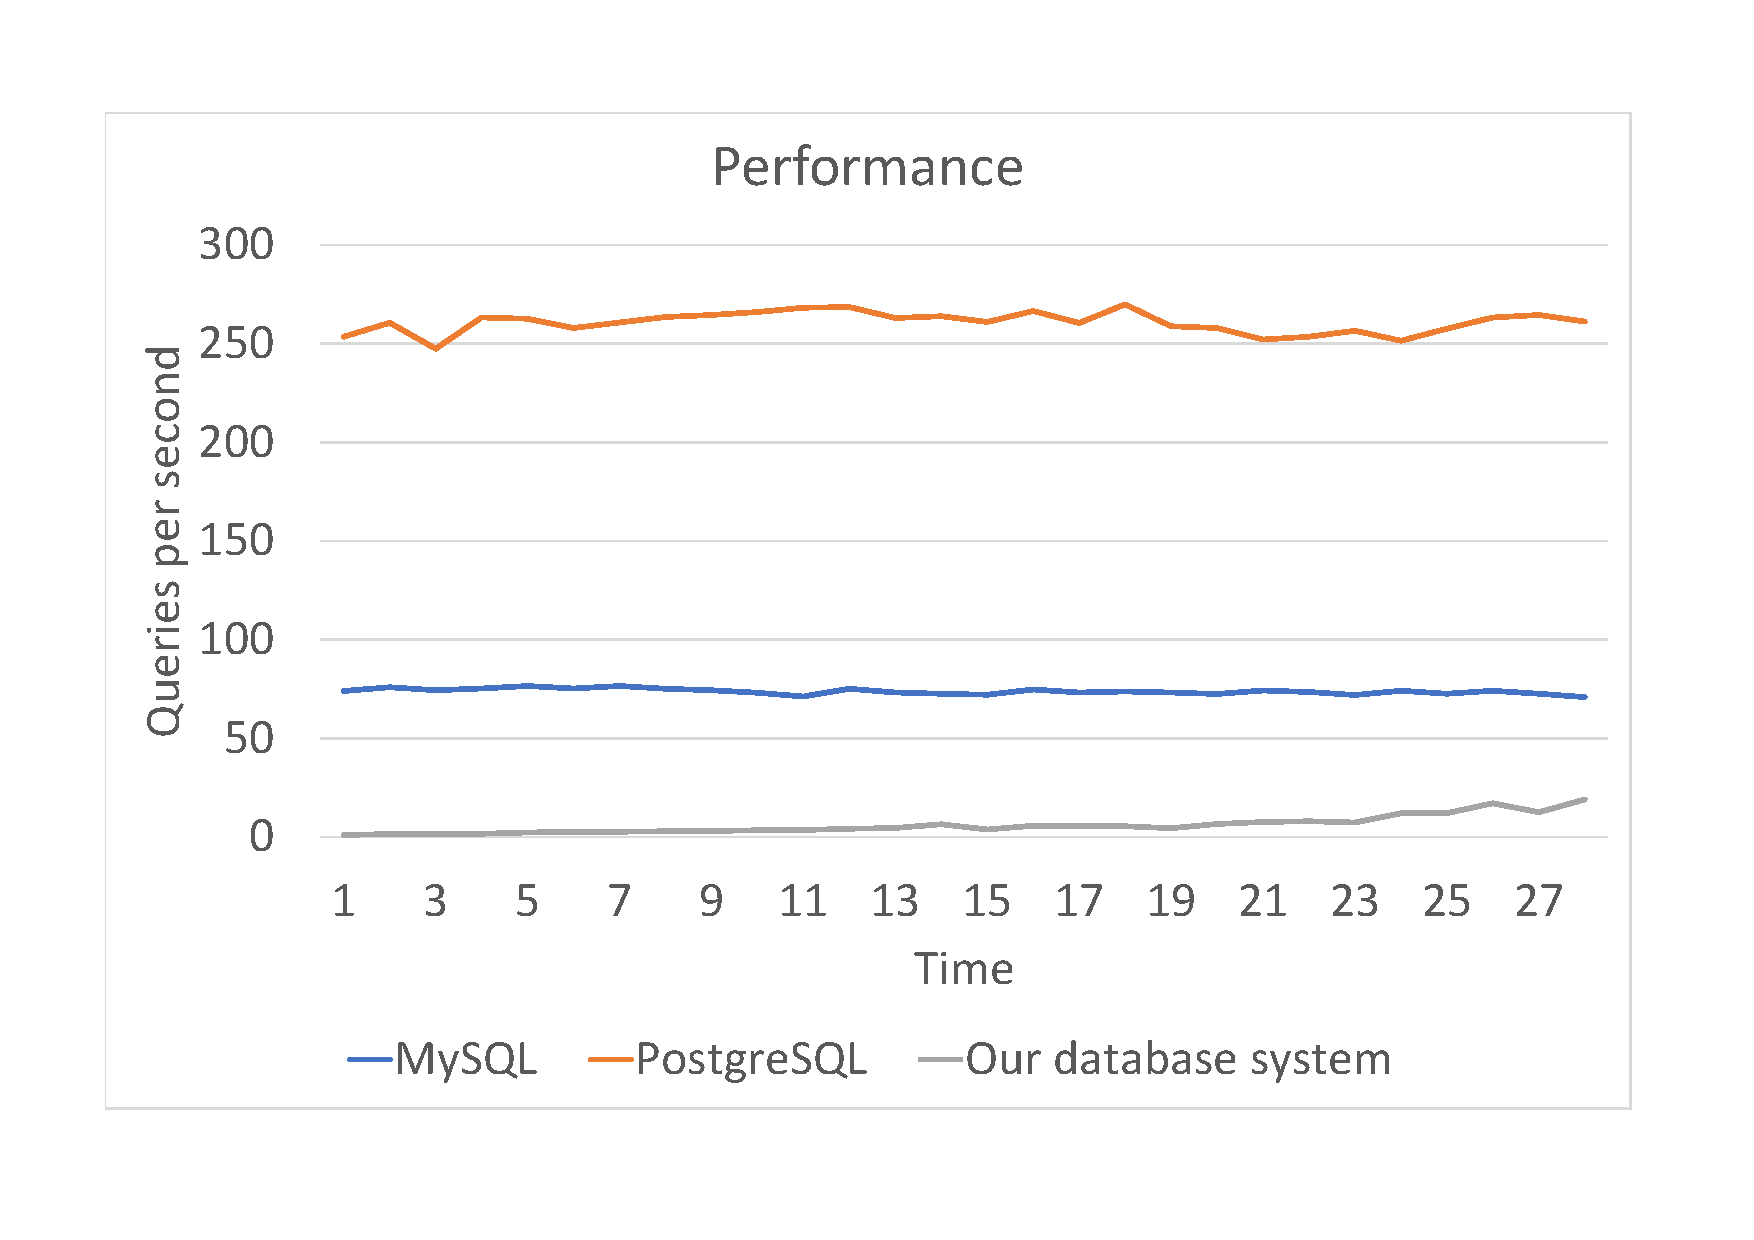
\includegraphics[trim={1.78cm 2cm 2.08cm 1cm},clip,width=1.0\linewidth]{excel/1per.pdf}
        \caption{Performance}
        \label{bench1per}
    \end{subfigure}
    \begin{subfigure}{.5\textwidth}
        \centering
        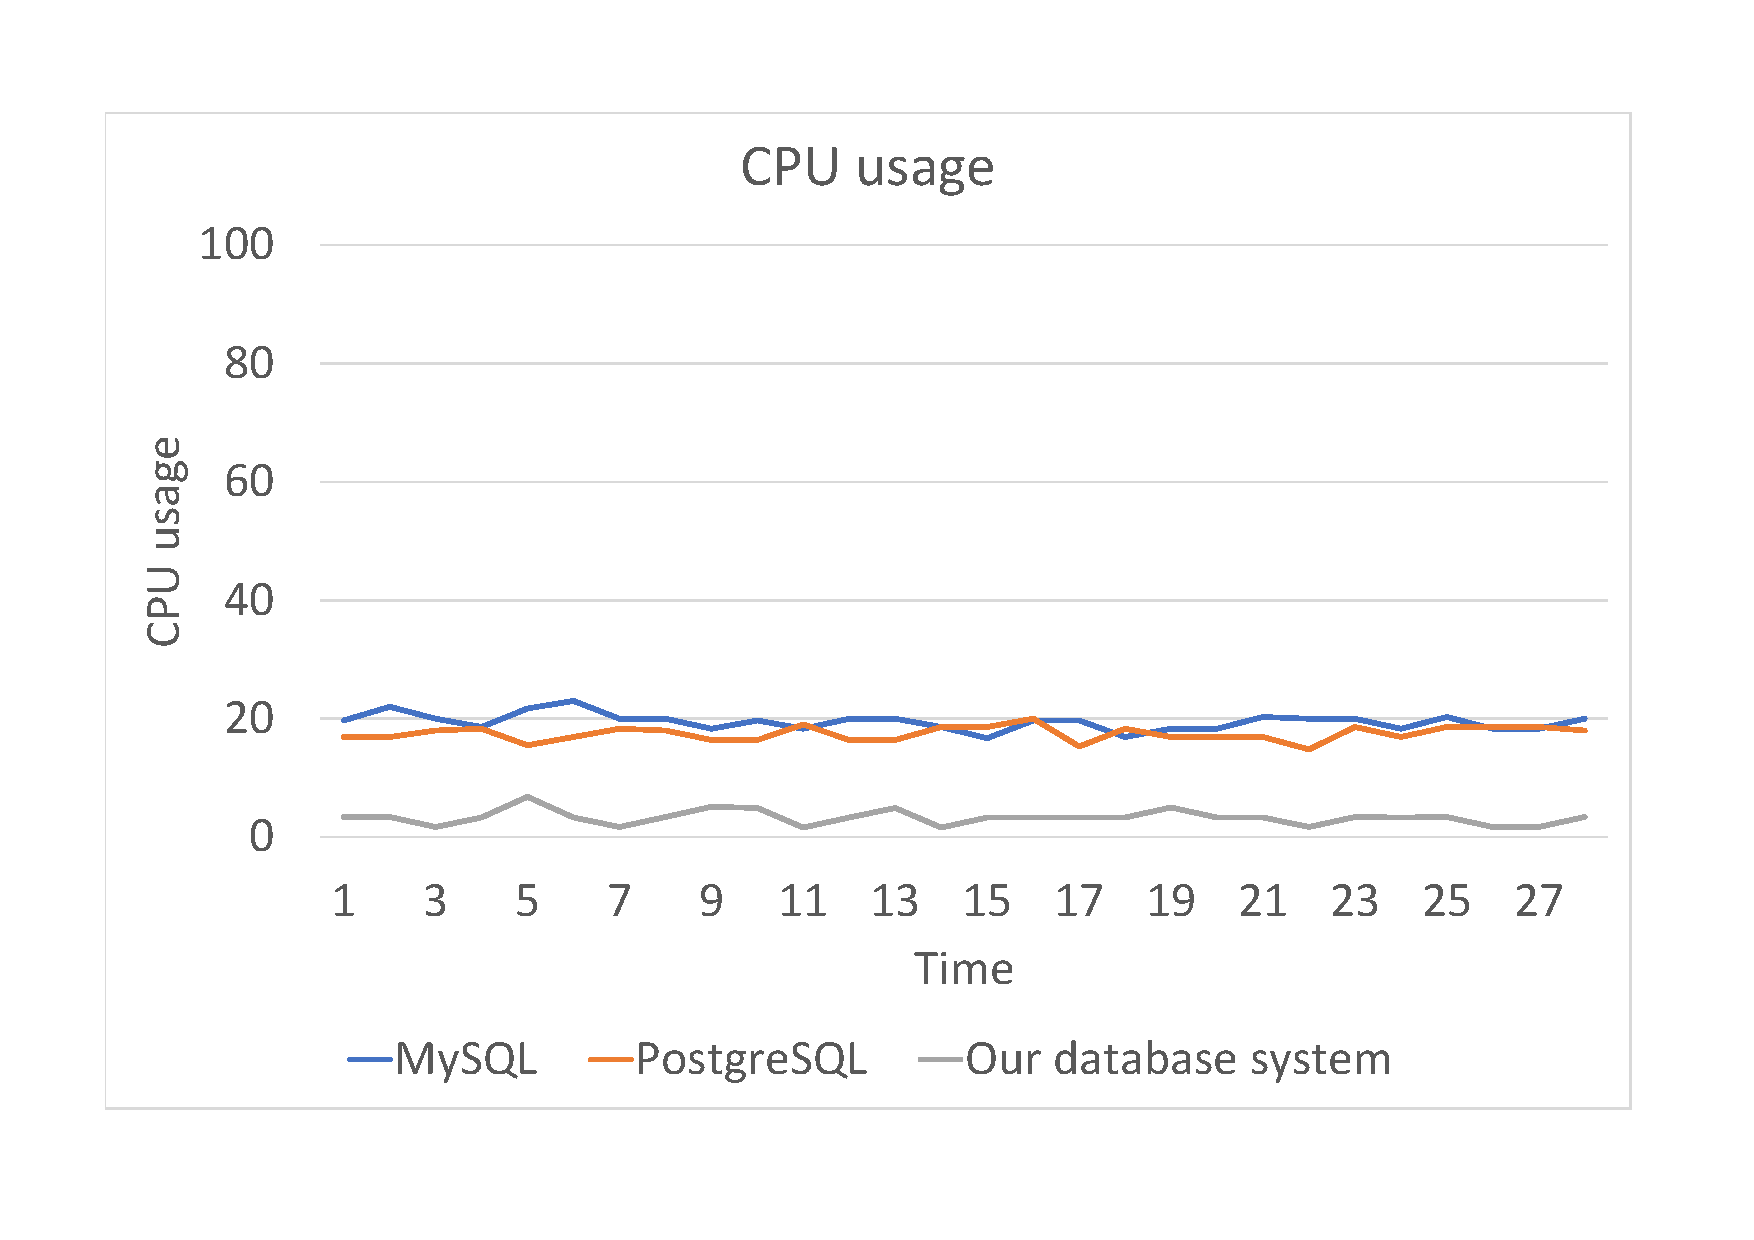
\includegraphics[trim={1.78cm 2cm 2.08cm 1cm},clip,width=1.0\linewidth]{excel/1cpu.pdf}
        \caption{CPU usage with}
        \label{bench1cpu}
    \end{subfigure}
    \caption{Single connected client benchmark plots}
\end{figure}



\subsubsection*{20 Connected Clients}
With 20 connected clients, PostgreSQL performance dropped to 50 queries per seconds and MySQL to 10 queries per seconds. At the end of benchmarking, our database system is more powerful than PostgreSQL and MySQL, because data gets distributed to clients (see \ref{bench20per}). Our database system also requires less processor time thanks to p2p network. Data are not obtained only from the server (as opposed to MySQL and PostgreSQL) but also from other clients. Thanks to this, our platform only using less than 20\% CPU power (see Figure \ref{bench20cpu}).

\begin{figure}[h]
    \begin{subfigure}{.5\textwidth}
        \centering
        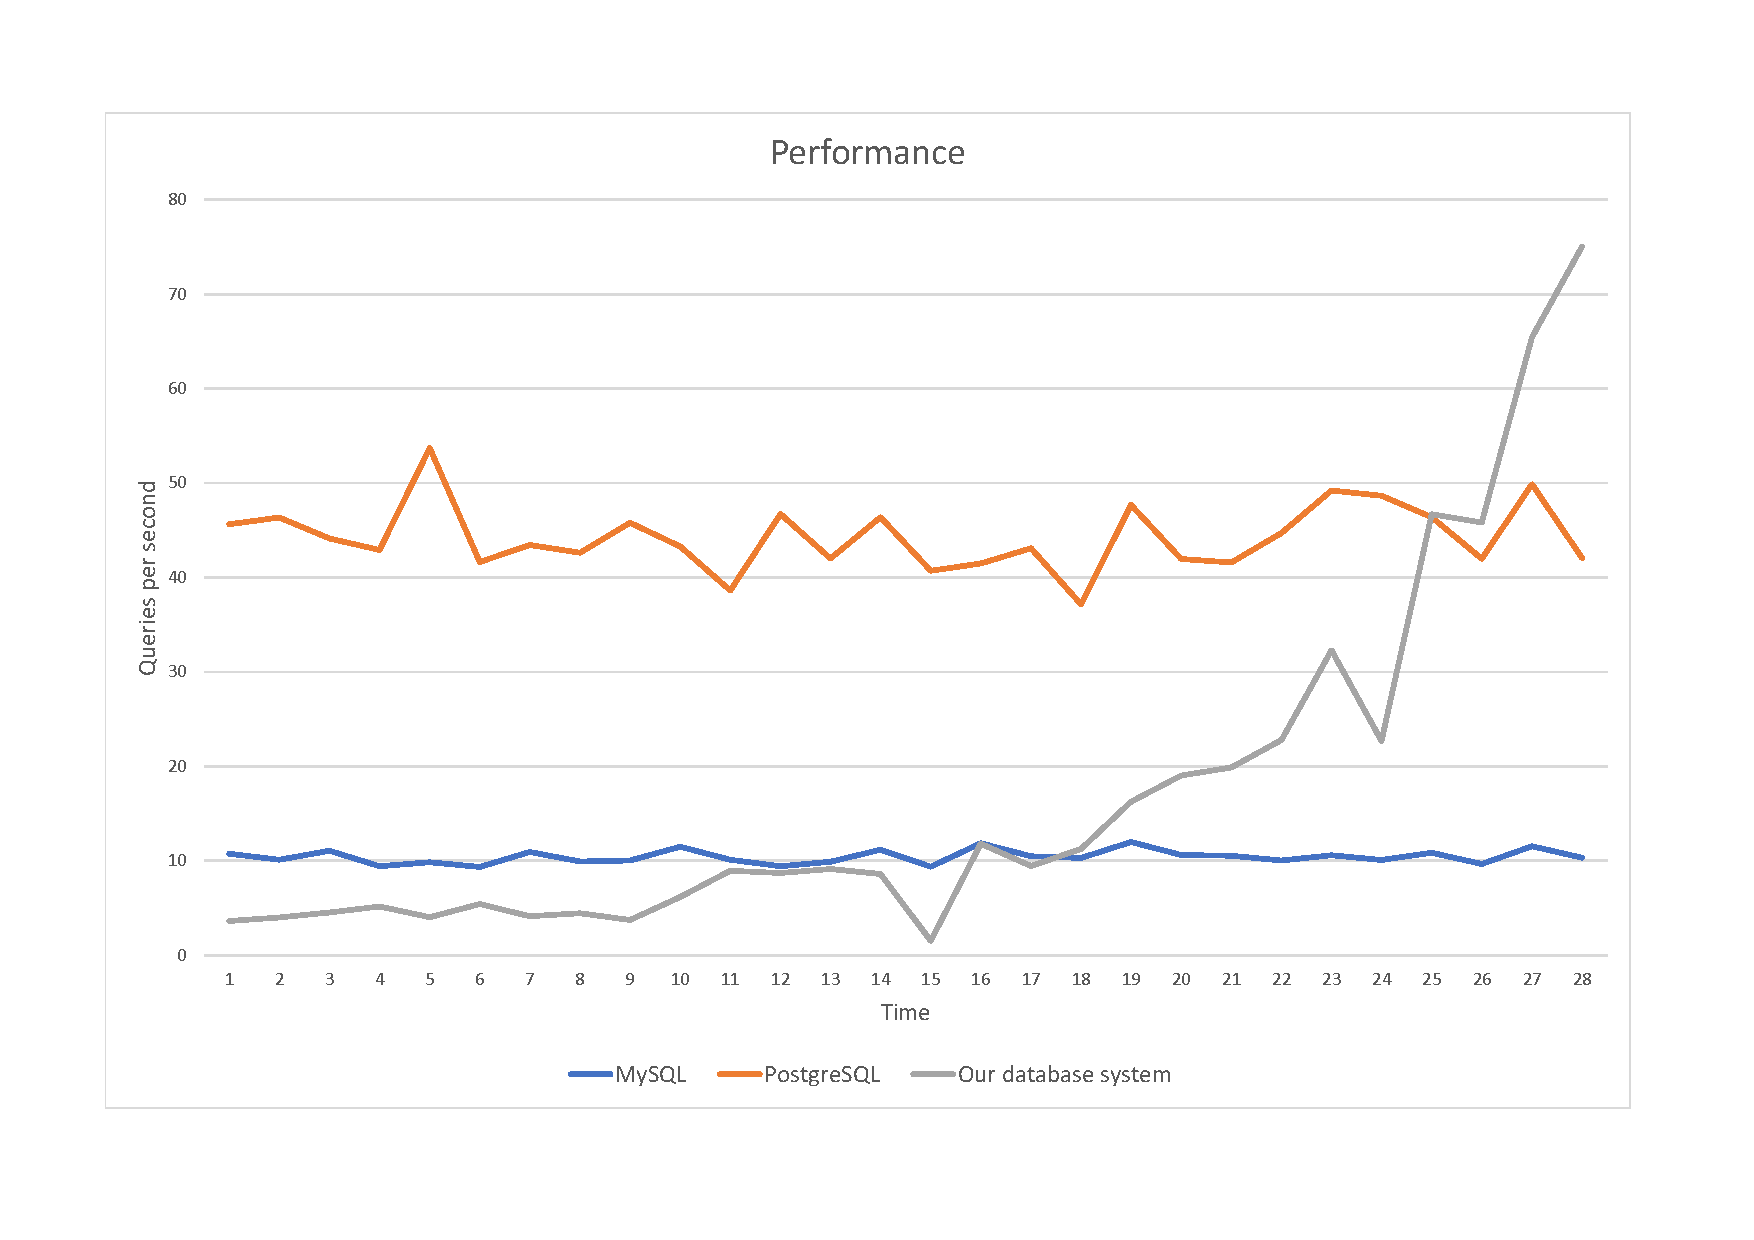
\includegraphics[trim={1.78cm 2cm 2.08cm 1cm},clip,width=1.0\linewidth]{excel/20per.pdf}
        \caption{Performance}
        \label{bench20per}
    \end{subfigure}
    \begin{subfigure}{.5\textwidth}
        \centering
        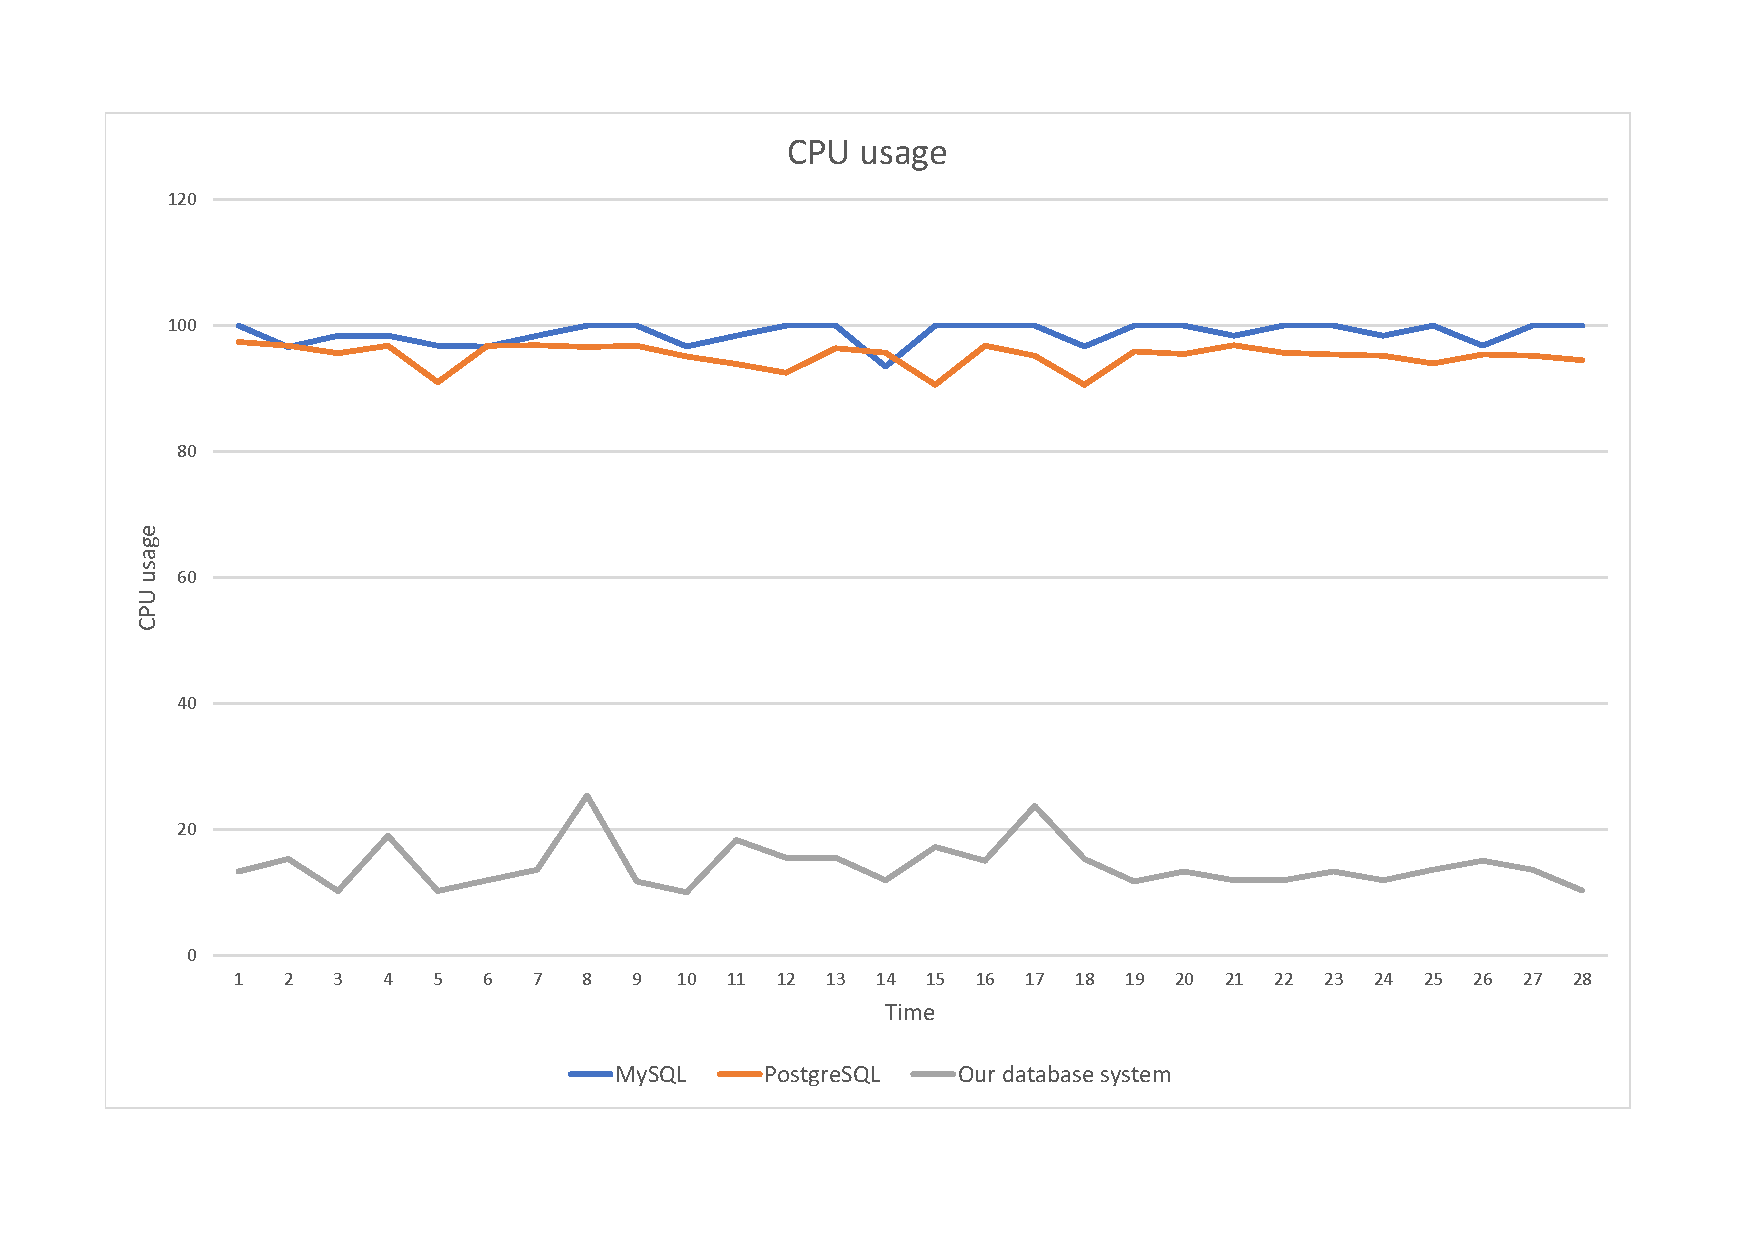
\includegraphics[trim={1.78cm 2cm 2.08cm 1cm},clip,width=1.0\linewidth]{excel/20cpu.pdf}
        \caption{CPU usage with}
        \label{bench20cpu}
    \end{subfigure}
    \caption{20 connected clients benchmark plots}
\end{figure}


\subsubsection*{80 Connected Clients}
With 80 connected clients, our database system outperforms MySQL and PostgreSQL after few seconds. Every client of our database system performs 100 queries per second. PostgreSQL client performs only 10 queries per second and MySQL only 2 queries per second (see \ref{bench80per}). CPU usage is in our database system also very low. In the beginning, when content is not distributed on the clients, the central node uses 60\% of CPU, but it decreases over time (see \ref{bench80cpu}).


\begin{figure}[h]
    \begin{subfigure}{.5\textwidth}
        \centering
        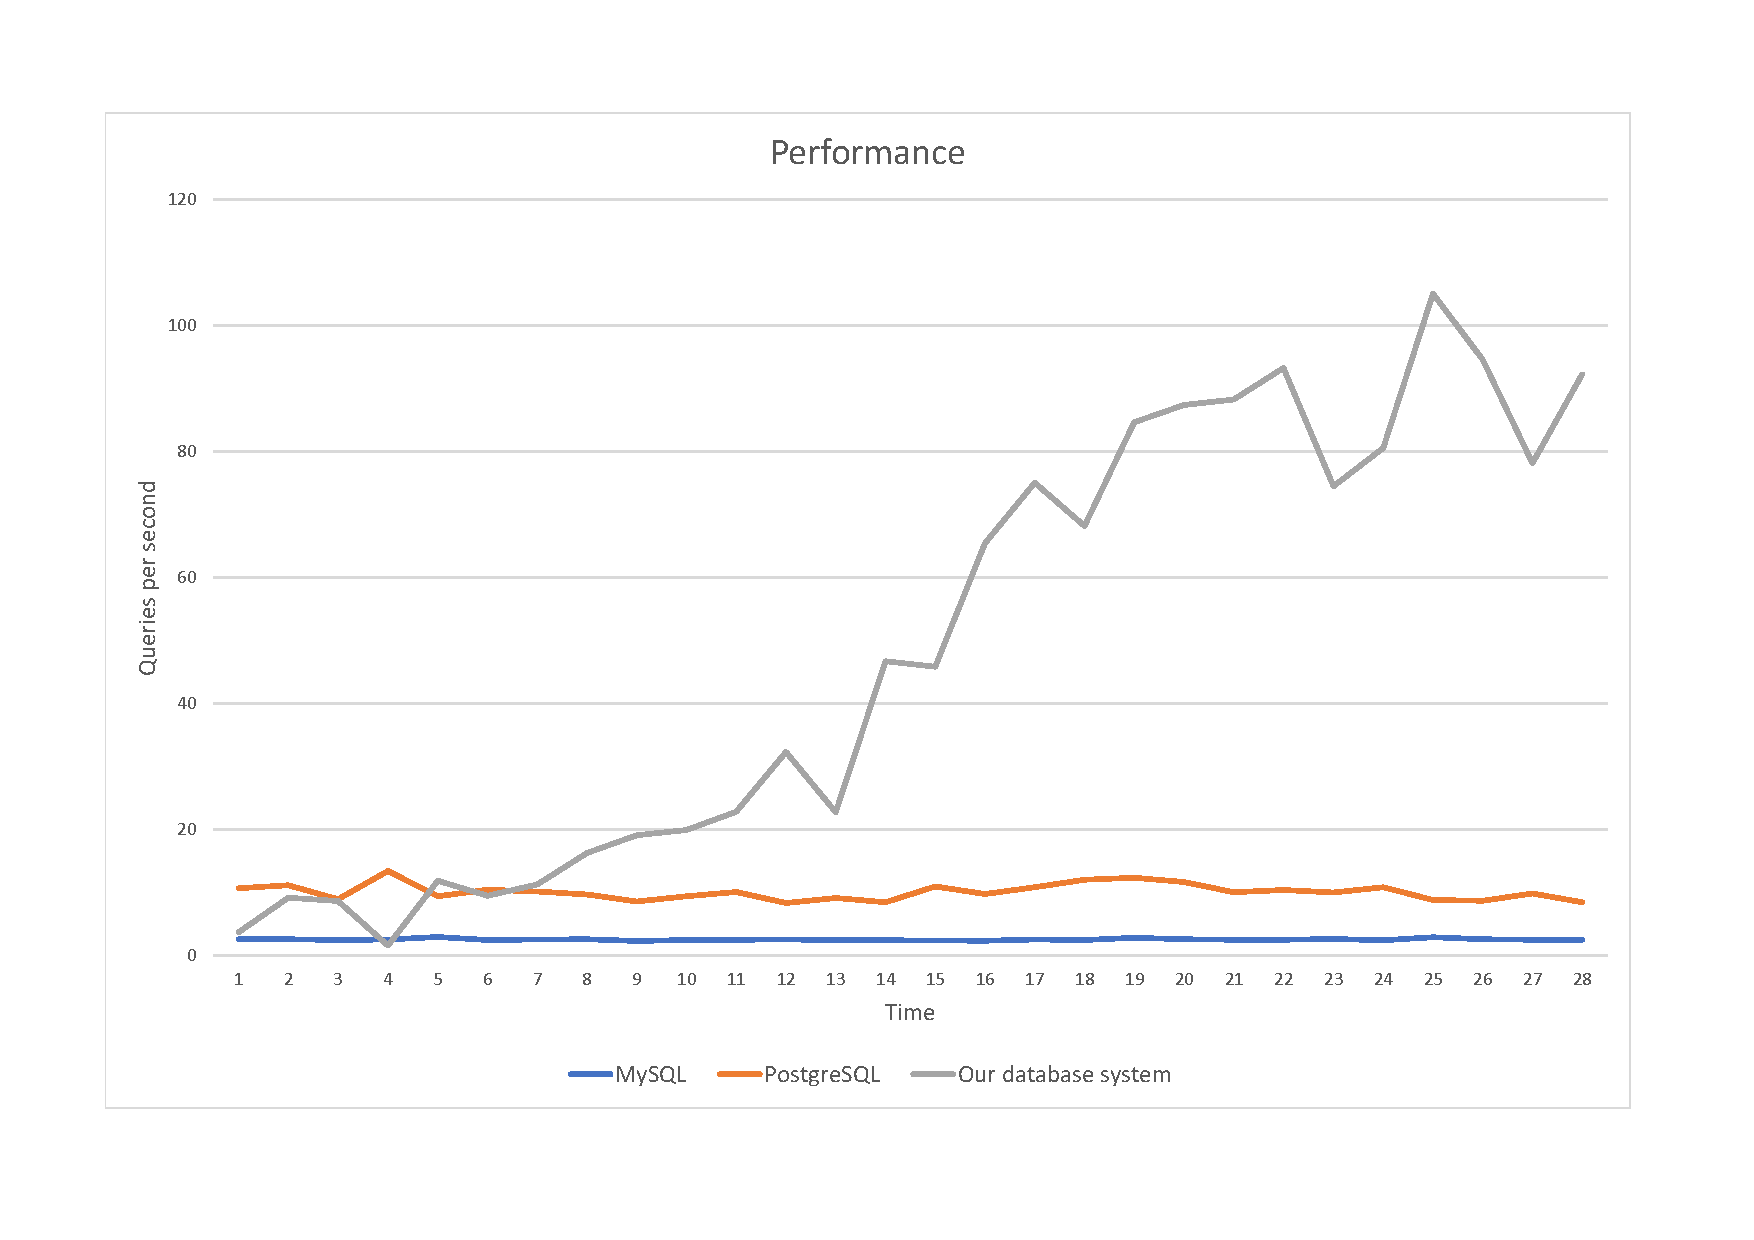
\includegraphics[trim={1.78cm 2cm 2.08cm 1cm},clip,width=1.0\linewidth]{excel/80per.pdf}
        \caption{Performance}
        \label{bench80per}
    \end{subfigure}
    \begin{subfigure}{.5\textwidth}
        \centering
        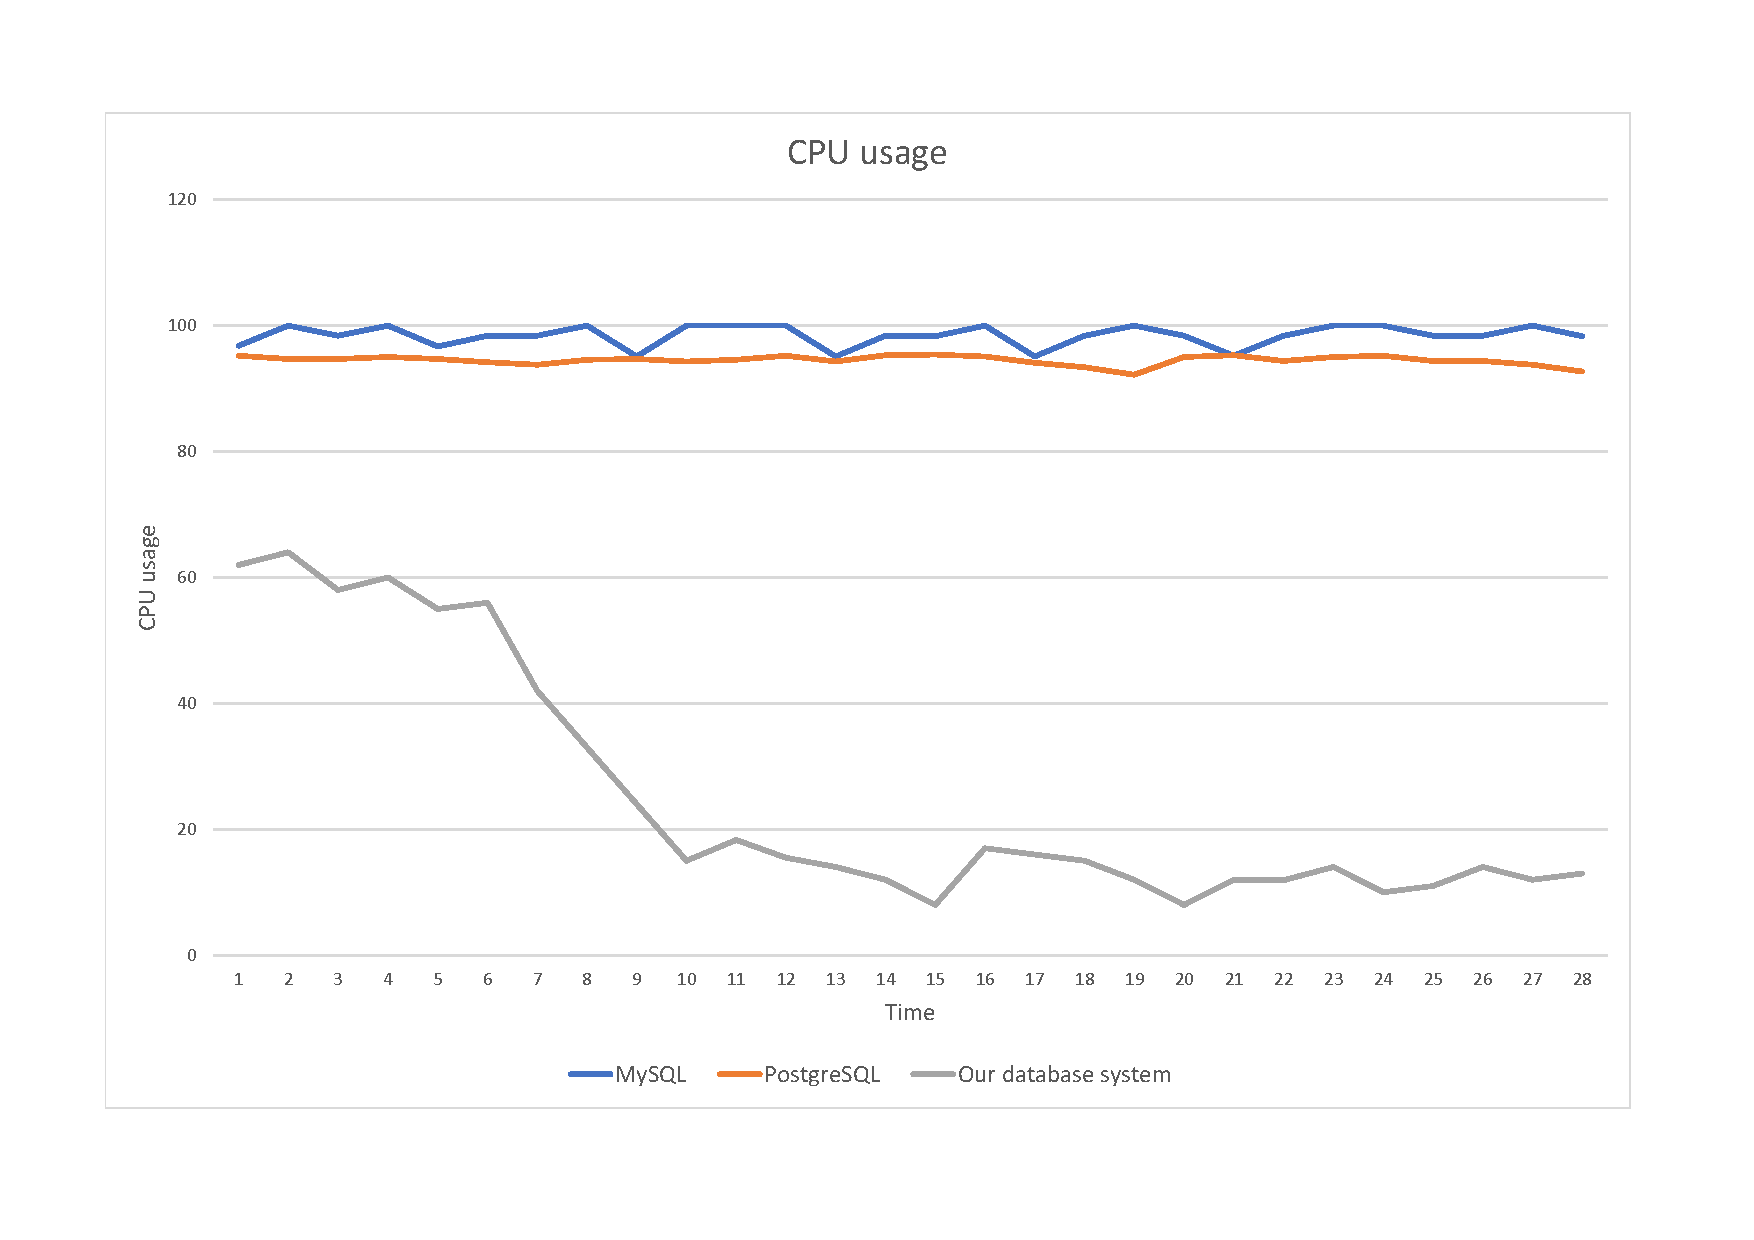
\includegraphics[trim={1.78cm 2cm 2.08cm 1cm},clip,width=1.0\linewidth]{excel/80cpu.pdf}
        \caption{CPU usage with}
        \label{bench80cpu}
    \end{subfigure}
    \caption{80 connected clients benchmark plots}
\end{figure}


\subsubsection*{150 Connected Clients}
We need to change the default PostgreSQL setting for maximum connections to connects more than 100 clients to the PostgreSQL. Our platform can handle 150 clients very well (opposite to MySQL and PostgreSQL). Each client connected to our database system can make up to 150 queries per second, and it increases by the time (see \ref{bench150per}). For the first seconds, CPU usage on the central node is high (near 100\%), but it decreases over time (see \ref{bench150cpu}).

\begin{figure}[h]
    \begin{subfigure}{.5\textwidth}
        \centering
        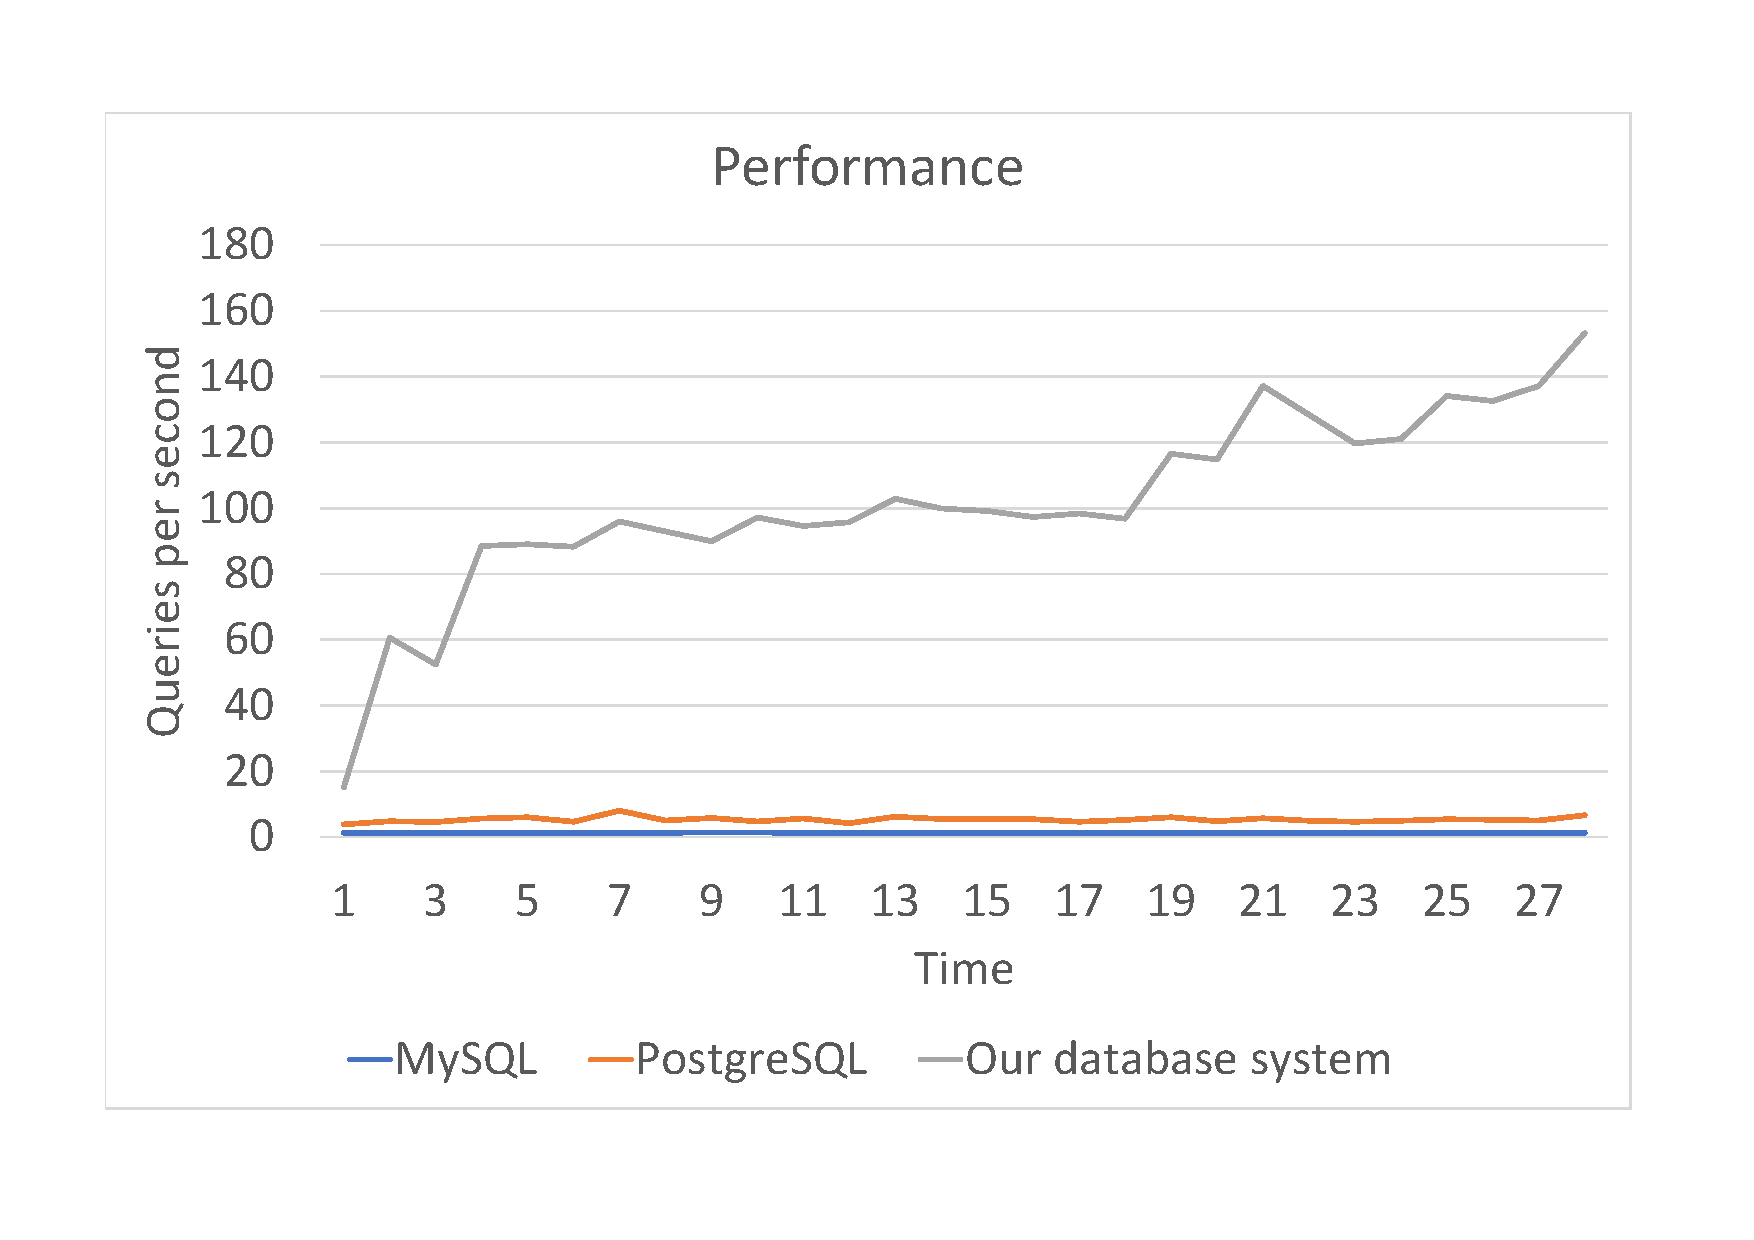
\includegraphics[trim={1.78cm 2cm 2.08cm 1cm},clip,width=1.0\linewidth]{excel/150per.pdf}
        \caption{Performance}
        \label{bench150per}
    \end{subfigure}
    \begin{subfigure}{.5\textwidth}
        \centering
        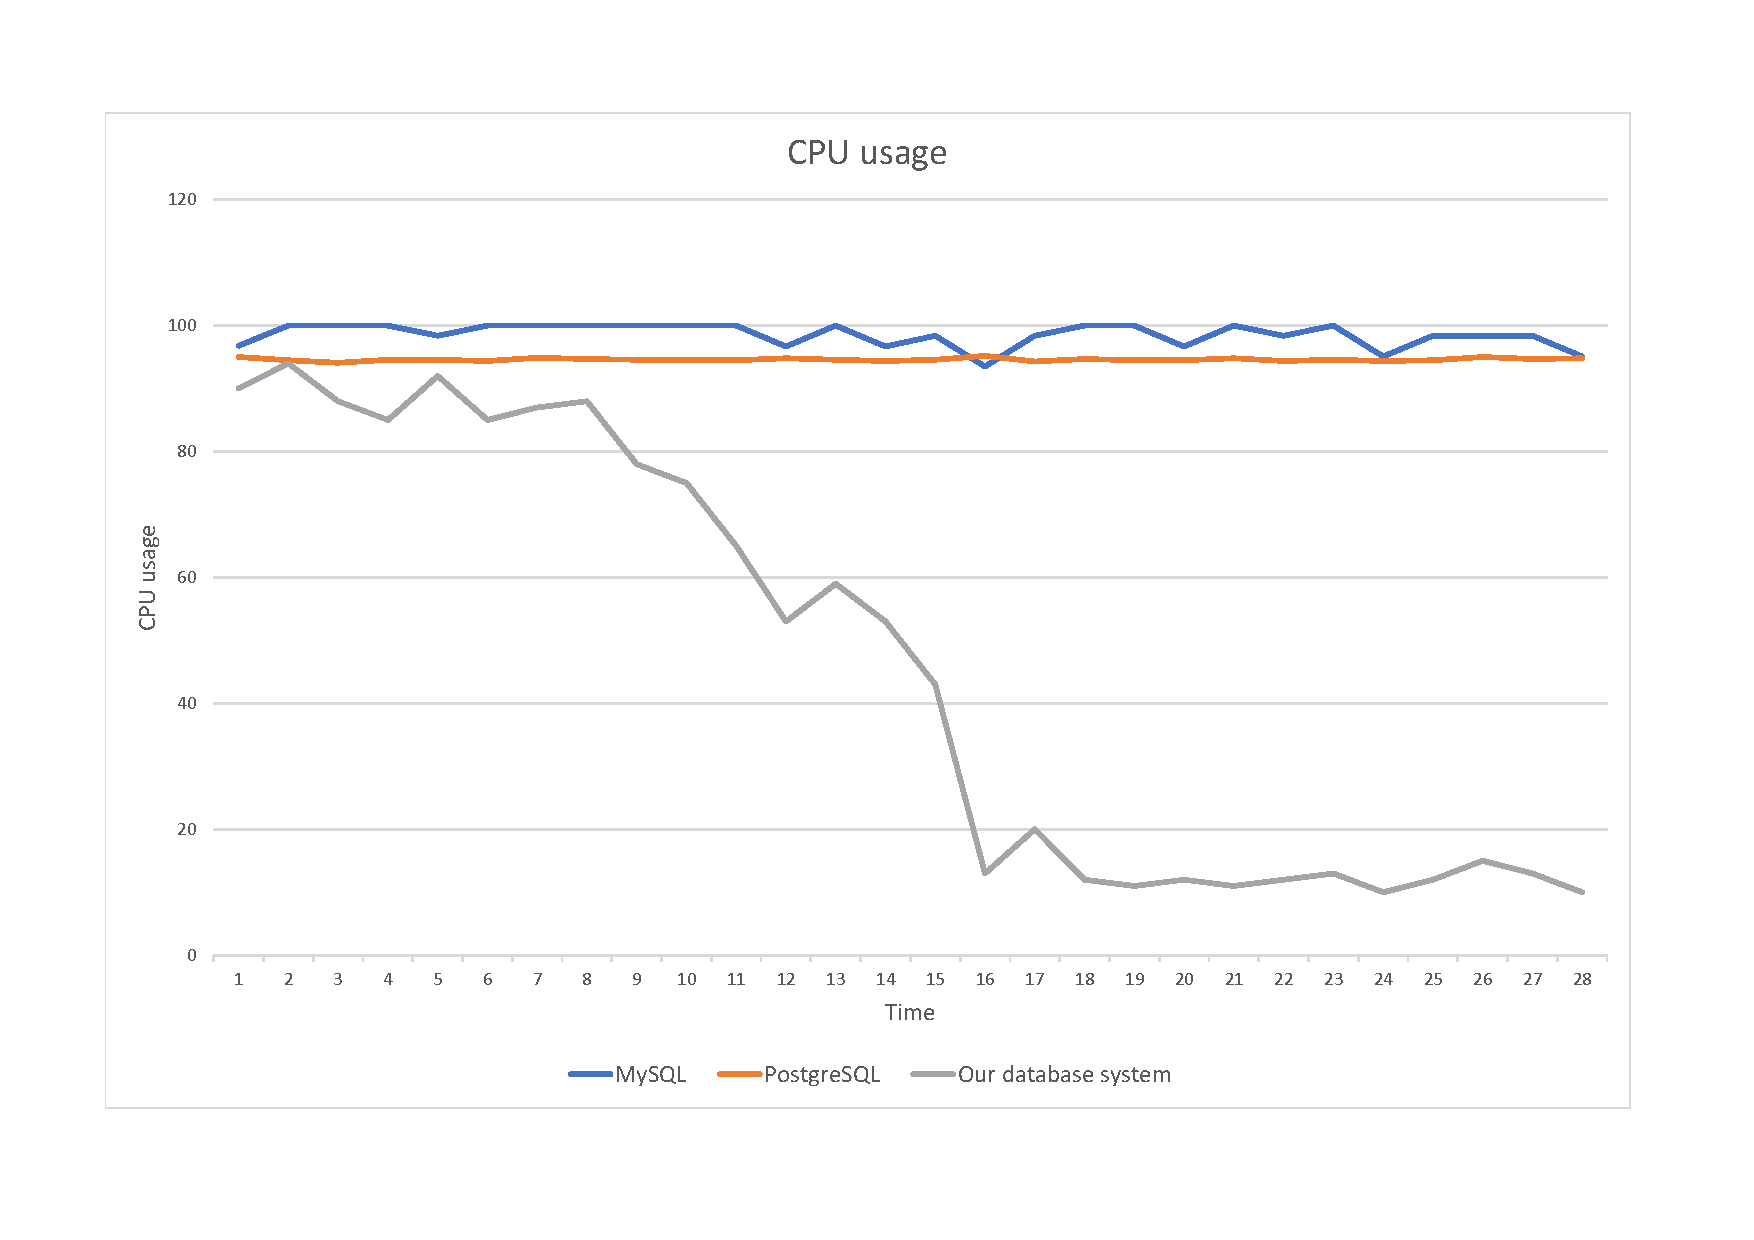
\includegraphics[trim={1.78cm 2cm 2.08cm 1cm},clip,width=1.0\linewidth]{excel/150cpu.pdf}
        \caption{CPU usage with}
        \label{bench150cpu}
    \end{subfigure}
    \caption{150 connected clients benchmark plots}
\end{figure}

\subsubsection{Benchmark Conclusion}
We can see that with more than 20 connected clients, our database system became more effective than traditional ones. Thanks to IPFS and its p2p network, a content of the database is distributed on the clients. This reduces the load on the central node.

\section{Comparing with Blockchain Explorers}
Our blockchain exploration platform is unique and differs from traditional blockchain explorers in many ways. See the table \ref{comparingTable} to compare traditional blockchain explorers with ours. 

\begin{table}
    \centering
    \begin{tabular}{| p{.2\textwidth} | p{.3\textwidth} | p{.3\textwidth} |}
    \hline
    & \textbf{Our platform}                                                                    & \textbf{Traditional blockchain explorer (Blockbook, Insight)}      \\ \hline
    Database system               & Proprietary                                                                         & Typically NoSQL database                                                        \\ \hline
    Views for blocks, transactions and addresses               & Yes                                                                         & Yes                                                        \\ \hline
    Complex queries support               & \textbf{Yes}                                                                         & No                                                        \\ \hline
    Filtering                             & \textbf{Yes}                                                                         & No, but filtering can be made by cycling over results     \\ \hline
    Sorting                               & \textbf{Yes}                                                                         & No                                                        \\ \hline
    Blockchain synchronization            & Typically slower but it depends on how many Feeders are working on blockchain & \textbf{Faster}                                                    \\ \hline
    Get block/transaction/address by hash & Slower                                                                        & \textbf{Faster, but may slow down if multiple nodes are connected} \\ \hline
    When more user is connected           & \textbf{Works faster}                                                                  & Works slower                                              \\ \hline
    Multiple coins support                & Yes                                                                          & Yes                                                \\ \hline
    \end{tabular}
    \caption{Comparing our platform with typical blockchain explorers}
    \label{comparingTable}
\end{table}

